\documentclass[manuscript, review, screen]{acmart}

\def\BibTeX{{\rm B\kern-.05em{\sc i\kern-.025em b}\kern-.08emT\kern-.1667em\lower.7ex\hbox{E}\kern-.125emX}}

% These commands are for a PROCEEDINGS abstract or paper.
\copyrightyear{2019}
\acmYear{2019}
\setcopyright{acmlicensed}

\begin{document}

\title{Real-time Twitter trends extraction and visualization system}

\author{Han Weng}
\authornote{Both authors contributed equally to this work.}
\email{h5weng@uwaterloo.ca}
\author{Hao Dong}
\authornotemark[1]
\email{h45dong@uwaterloo.ca}
\authornote{From section CS631}
\affiliation{%
  \institution{University of Waterloo}
  \city{Waterloo}
  \state{Ontario}
  \postcode{N2L0E1}
}


\renewcommand{\shortauthors}{H. Weng and H. Dong (CS631)}

\begin{abstract}
In this project, we anticipate to build a simple ``twitter'' engine to support extracting trends based on some real-time tweets data. We start with a tweet data set containing 1.6 million data, which is randomly written to a logger and provided to Flume. Flume then works as the producer for a Kafka broker to which Spark Streaming is connected. Finally the data is written to logs again which are read to Zeppelin where they are visualized real-time in an interactive way. We use this project as a simulation to real life scenarios by loading burst, imbalanced data producing/consuming and we hope to learn a full cycle of back-end data collection, processing and visualization from it. 
\end{abstract}

\keywords{big data, spark streaming}

\maketitle

\section{Introduction}
Twitter is one of the most commonly used social media nowadays and usually acts as a very important window by people to obtain the idea of public opinion very efficiently. Its succinct message form and wide acceptance make it possible to detect the outbreak news and bursty trend faster than ever. Therefore, there has been growing attention paid into information mining on tweet data. However, most work done by us before was on an OLAP basis. In this project, we also have a tweet data set which was studied by other researchers in a batch-processing way, but instead of digging further into the data, we put more attention to learning about the distributed architecture, real-time streaming and also spark visualization in this work. 

\section{Framework}

\subsection{Data source}
The data source we use is a tweet data set with 1.6 million records. These are real tweets sent between Apr 6 and Jun 16 in 2009. We also looked into twitter APIs to try to obtain real tweets for current time, but Twitter sets a limit on the number of requests in a certain window, which makes the number of tweets really low which does not meet our requirement for streaming. Also, in this project we care more about the process of message passing process and throughput in the architecture themselves but not data mining or language model building, so we decided to stick to the original data set to give us more flexibility. 

The data set contains timestamp, user-id and tweet. In addition to that, in order to make the visualization more meaningful and test the performance we added two additional columns: age and gender, which are simply random integers between 15 and 60 and random labels respectively. A python script is used to extract tweet as well as generate this information, which is written to a log file and monitored by a Flume instance. 

\subsection{Overview}

\begin{figure}
    \centering
    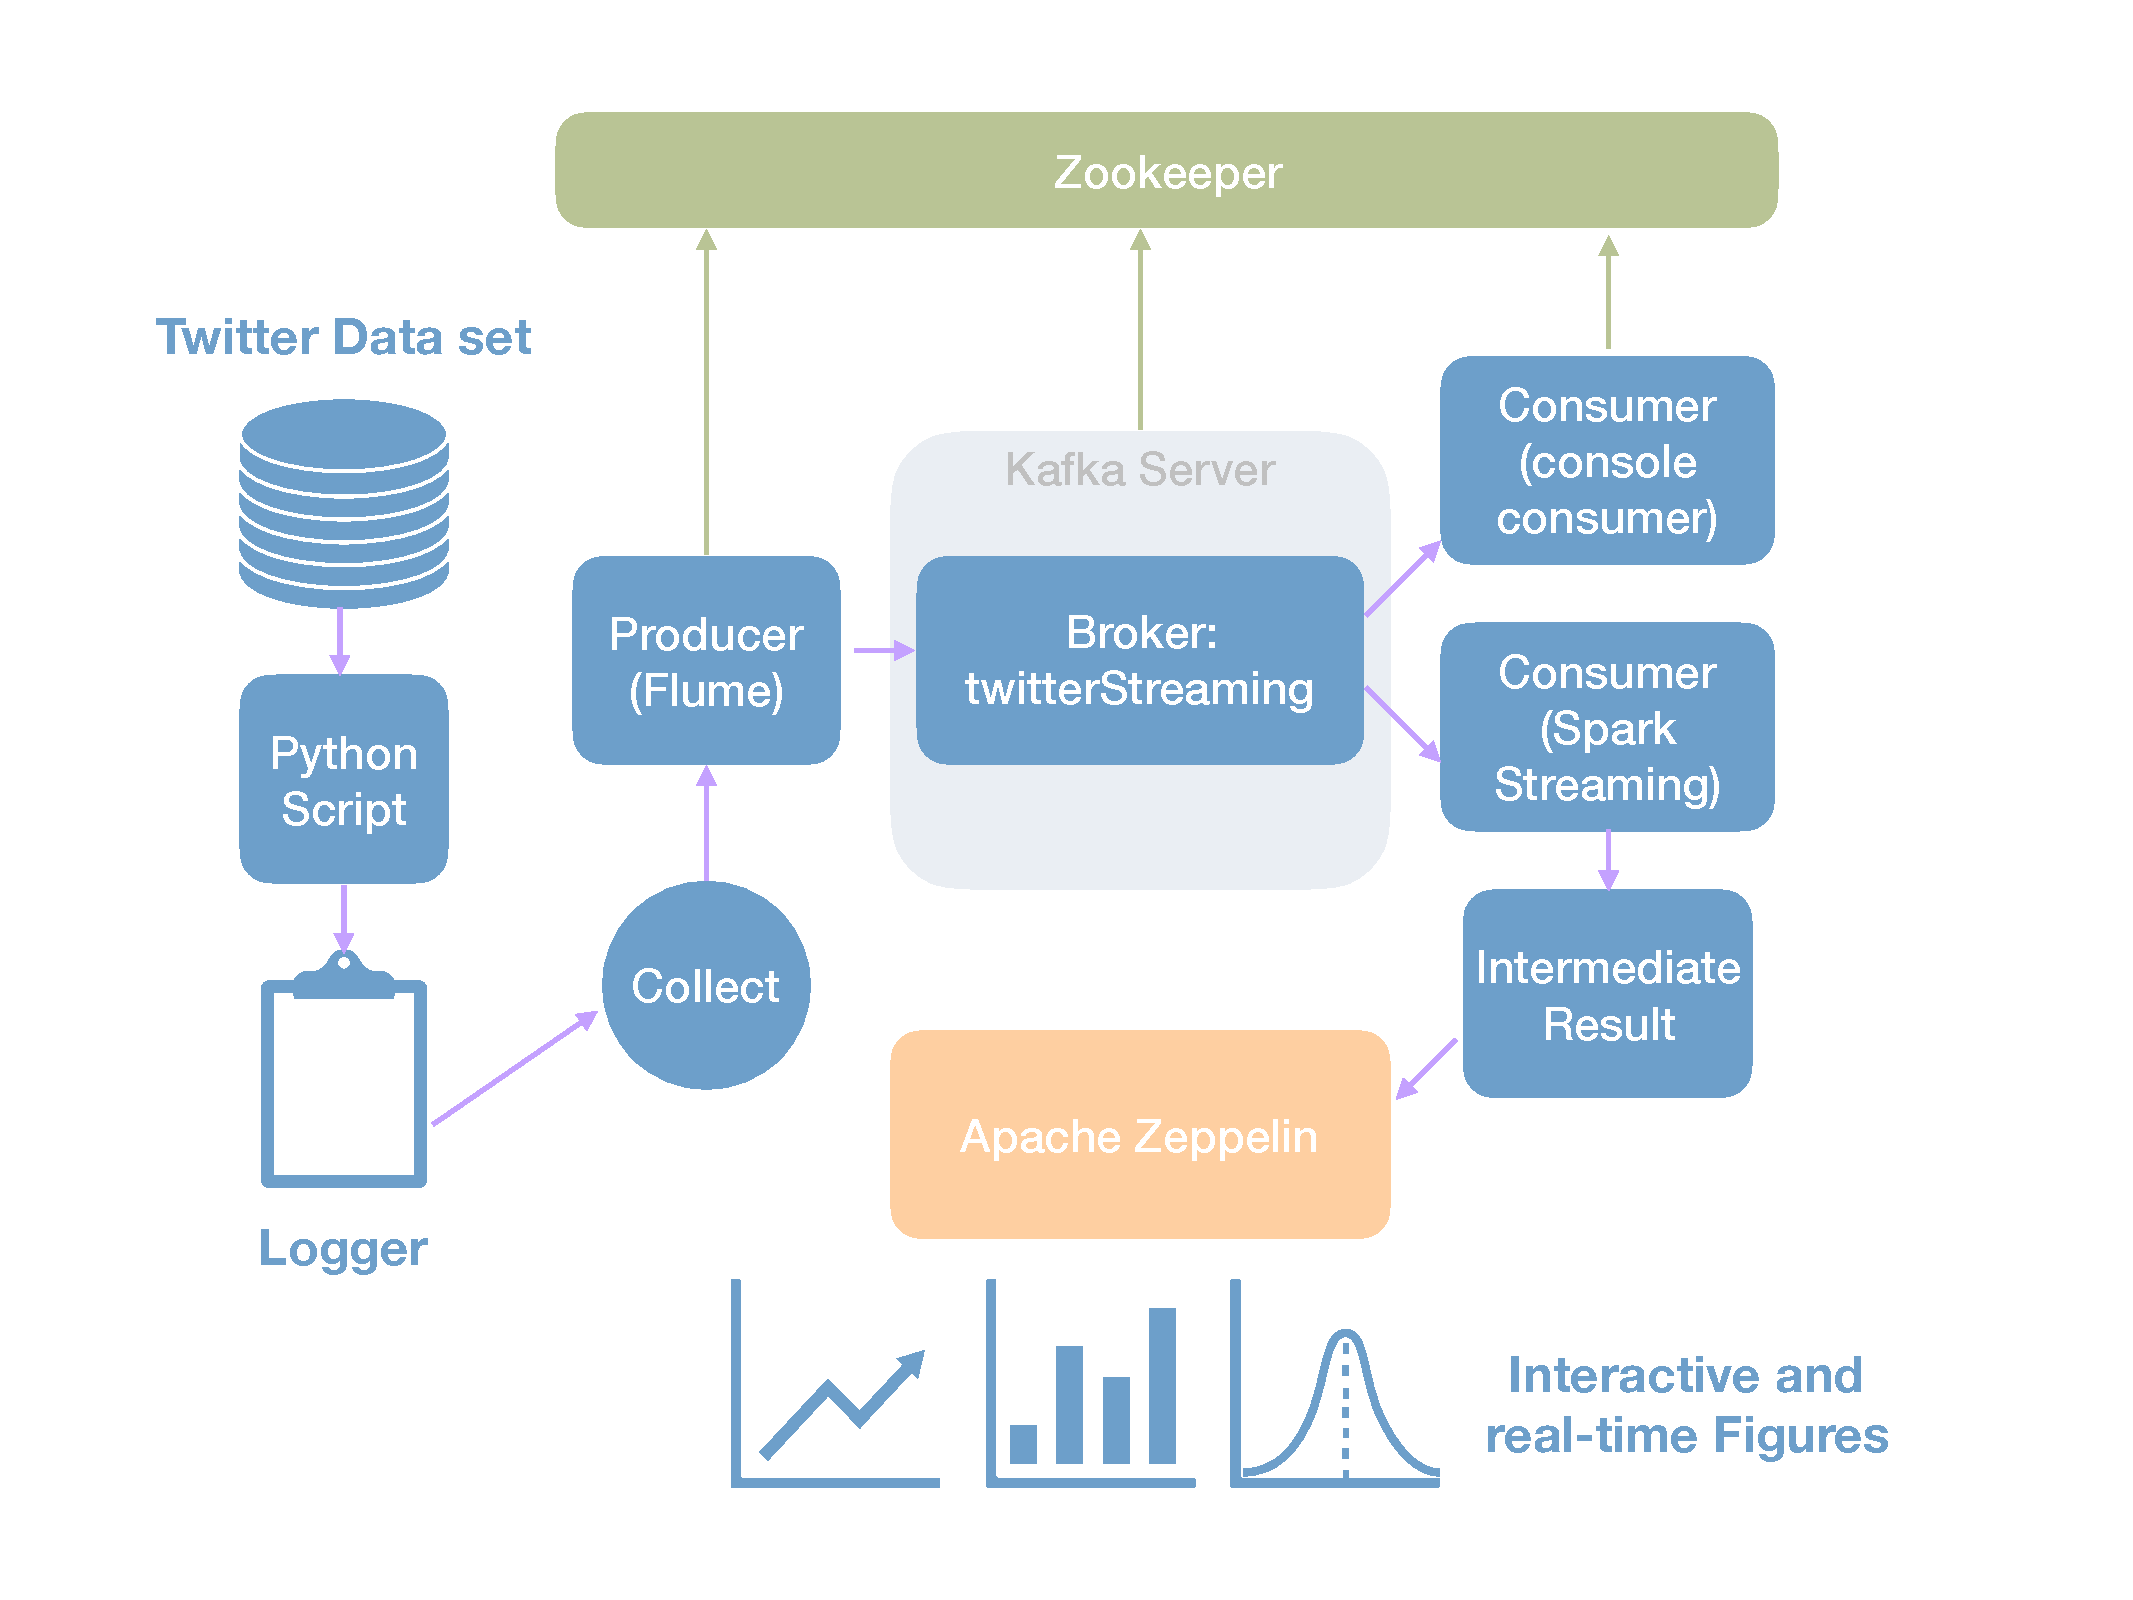
\includegraphics[width=\textwidth]{arch.pdf}
    \caption{General structure of the model.}
    \label{fig:arch}
\end{figure}

Fig. ~\ref{fig:arch} shows the framework we use in this project. We use the combination of Apache Flume and Apache Kafka as the data container to hold the incoming tweets before writing them to Spark Streaming. Flume is a distributed and reliable system to collect information from multiple sources and move them to a single center. It integrates very well with Kafka as a producer, then Kafka that processes the subscription events, sink the data collected to different brokers for us to consume. In this project, one broker with two consumers connected are used including one console consumer to test the throughput and for verification, while the other one sinks data to spark streaming, as can be seen from Fig. ~\ref{fig:arch}.

\subsection{Setup}
The server is started in the following sequence: ZooKeeper where the tasks are held, Kafka server, then the Flume producer. They are started with the following main parameters (only part of important ones are shown here):

ZooKeeper:
\begin{verbatim}
    tickTime=2000
    initLimit=10
    syncLimit=5
\end{verbatim}

Kafka:
\begin{verbatim}
    num.network.threads=3
    num.io.threads=8
    socket.send.buffer.bytes=102400
    socket.receive.buffer.bytes=102400
    socket.request.max.bytes=104857600
    ...
    num.partitions=1
    num.recovery.threads.per.data.dir=1
    ...
    group.initial.rebalance.delay.ms=0
\end{verbatim}

Flume:
\begin{verbatim}
    exec-memory-kafka.sinks.kafka-sink.type = org.apache.flume.sink.kafka.KafkaSink
    exec-memory-kafka.sinks.kafka-sink.brokerList = localhost:9092
    exec-memory-kafka.sinks.kafka-sink.topic = twitterStreaming
    exec-memory-kafka.sinks.kafka-sink.batchSize = 20
    exec-memory-kafka.sinks.kafka-sink.requireAcks = 1
\end{verbatim}

The environment is tuned to be successfully running in local mode so far, and we are still on the way to try running it in a distributed way.

\section{Spark streaming}
On top of the server, we connect Spark Streaming as a consumer to process the streaming data. The basic look of the program is similar to Assignment 7 in this course, doing some basic word frequency stats and twitter tag count. The streaming window setting is illustrated by Fig. ~\ref{fig:sparkstreaming}. We try to grasp the trend for every minute's tweets, updating every 5 seconds. As this is not an algorithm intensive project, and that the codes can be found in the project GitHub repository, we do not discuss much about the streaming process in this report. Overall, the program reads in streaming tweets as text, then splits and filters it to different output files, including word count (group by timestamps), "bulletin-board" word count (one file keeps updating and being overwritten by newest result), bigram count, bigram "bulletin-board", tag count and tag "bulletin-board". The one with timestamps is used later in the dashboard we build, and the one keeps refreshing is for the streaming plot.\

\subsection{Words filtering}

Regarding the word filtering, we use a word set defined by a built-in Scala library\\ \texttt{org.apache.spark.ml.feature.StopWordsRemover}, plus some frequently occuring words that observed in the results which we think does not make much sense. This ensures that stop words such as "I", "have" will be removed when doing trend stats. 

\begin{figure}
    \centering
    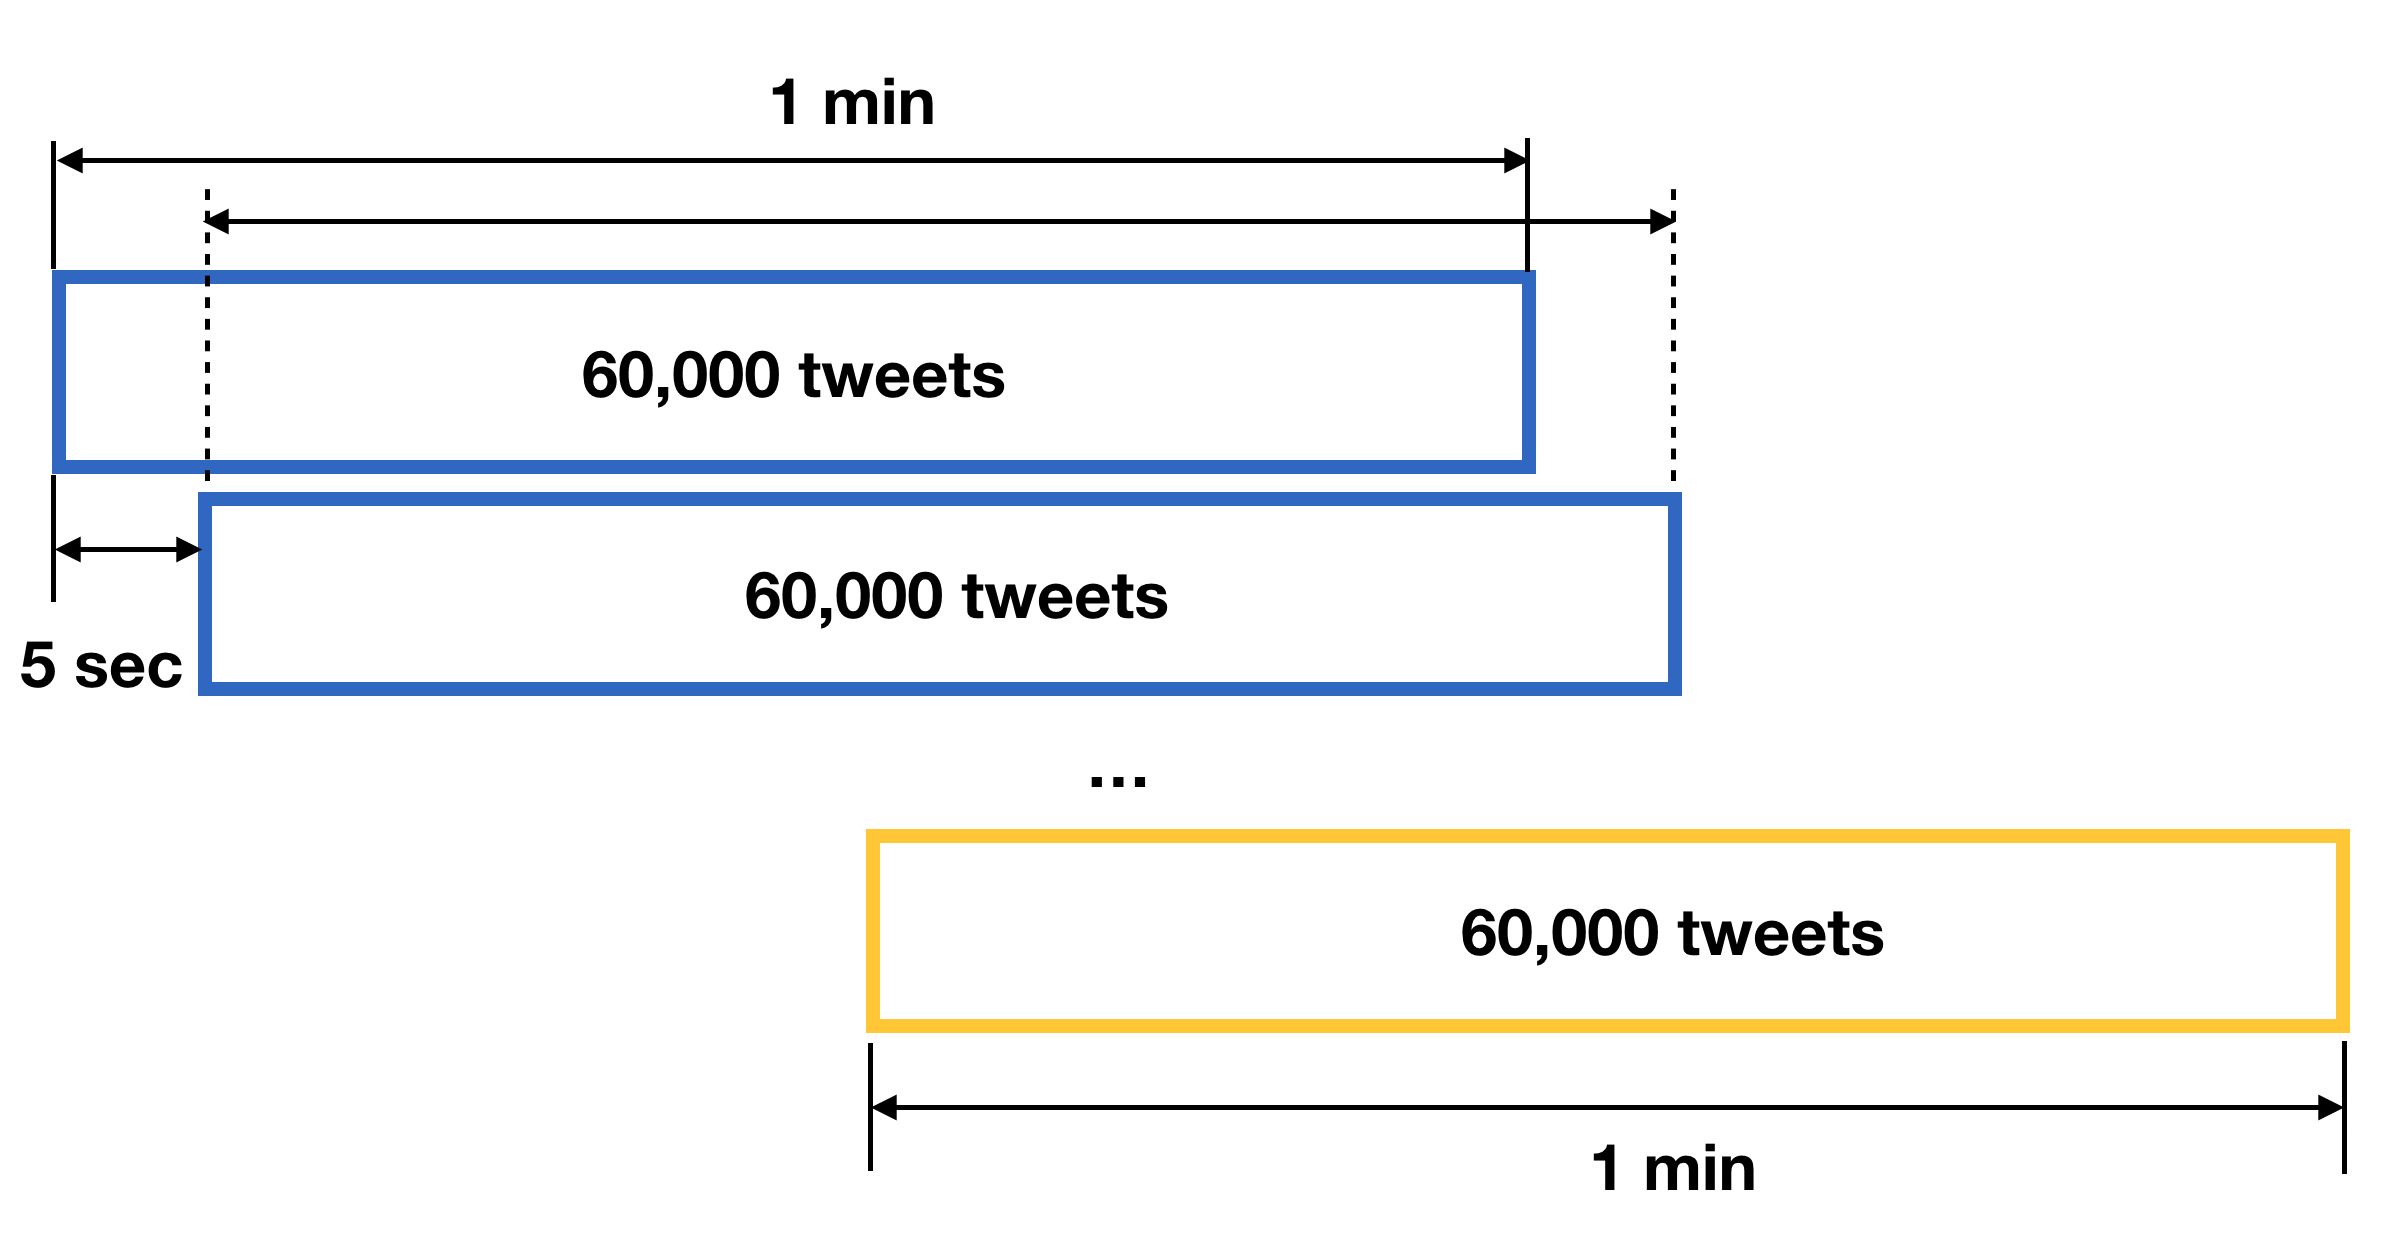
\includegraphics[width=5in]{sparkstreaming.png}
    \caption{Spark Streaming window settings}
    \label{fig:sparkstreaming}
\end{figure}

\subsection{Intermediate result}
We first stored the intermediate results on HDFS by storing mapped pairs to allow maximum plotting flexibility. However, we found that reading from HDFS then performing visualization in some our visualization frameworks become slow if the pass-in data exceeds some volume, causing significant lag in the streaming plotting. Therefore, we later switched to use local file system and read text files from it directly. One of the streaming plotting will trace file changes dynamically while the other needs manual script running (it is though automated through some JavaScript trick, but still not in-place refreshing like true streaming), which will be introduced in more details in the next section.

\section{Visualization}
We explored multiple streaming visualization frameworks and looked further into a few of them, including lightning-viz\footnote{http://lightning-viz.org/}, highcharts\footnote{Live data from CSV can be done as https://www.highcharts.com/demo/live-data} and Apache Zeppelin. The factors we take into consideration when doing this are we expect the visualization to be real-time (to reflect streaming data), and interactive (to make it dynamic and flexible for user needs). Lightning-vis is based on D3, a popular JavaScript plotting library and it creates most fabulous figures, but lacks interactive interface and the complex dependency makes its application restricted within the it's own server. Highchart has better interactivity than lightning-vis, but it only allows mouse interaction with data points instead of flexible control.

A satisfactory interactive solution is Apache Zeppelin. This is a novel visualization platform which has built-in spark support. By creating \texttt{DataFrame} objects in Spark, it allows very flexible plotting by Spark SQL with interactive selection and input feature. Further more, it even allows customizing chart content by simply dragging-in and out features, and has not bad integration with streaming data.

To implement both streaming plotting and interactive dashboard, we decided to use the combination of lightning-viz and Apache Zeppelin for different tasks.

\subsection{V1. Word/Tag trend streaming plotting}
As discussed above we implemented the streaming plotting using lightning-viz. This is a framework running on a local server with a web interface, which dynamically shows the trend of each word/tag with time by reading in the newest files from the intermediate results. New data is continuously written to the plotting data collection and plot is refreshed real-time as new data added in. Fig. ~\ref{fig:streaming-vis} shows how it looks, but since this report is PDF it only shows a static image of one frame. The animated image can be found in the README file from the git repository of this project.

\begin{figure}
    \centering
    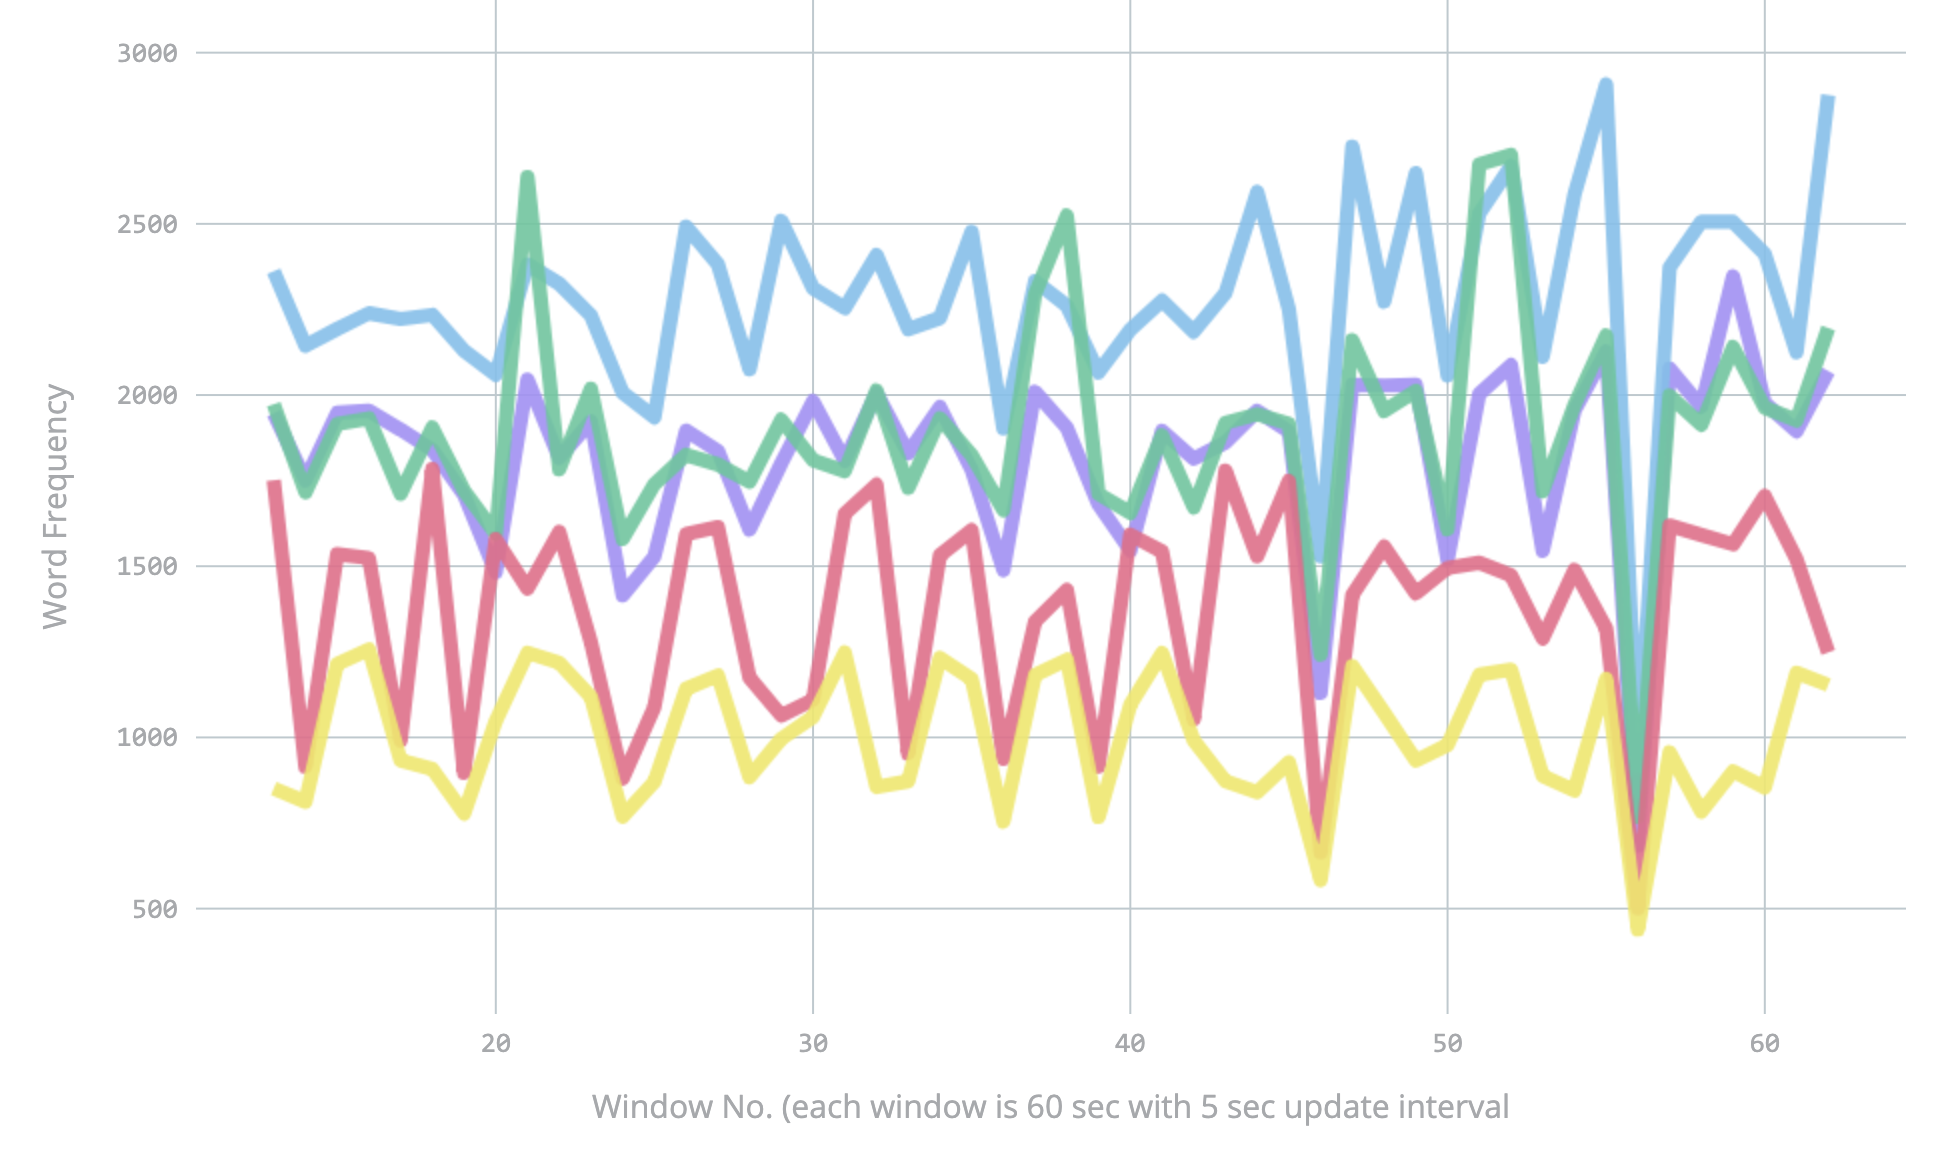
\includegraphics[width=5in]{streamingplot.png}
    \caption{Screenshot of the streaming visualization. Only one frame shown here. The animated file can be found in the README.md file in the git repository. The low point on the graph corresponds to the low server load time (less incoming data to stream).}
    \label{fig:streaming-vis}
\end{figure}

\subsection{V2. Interactive dashboard}
The interactive dashboard is implemented in Apache Zeppelin. The platform is designed to work with Spark and Spark Streaming and allows us to run any scala (in particular, spark), python and SQL code by configuring the corresponding interpreters. Fig. ~\ref{fig:dashboard} shows a preview of the dashboard. We have added 6 charts to it as demo, but new features can be easily included to the dashboard since we make the DataFrame quite flexible and also thanks to the powerful visualization ability of Zeppelin.

\begin{figure}
    \centering
    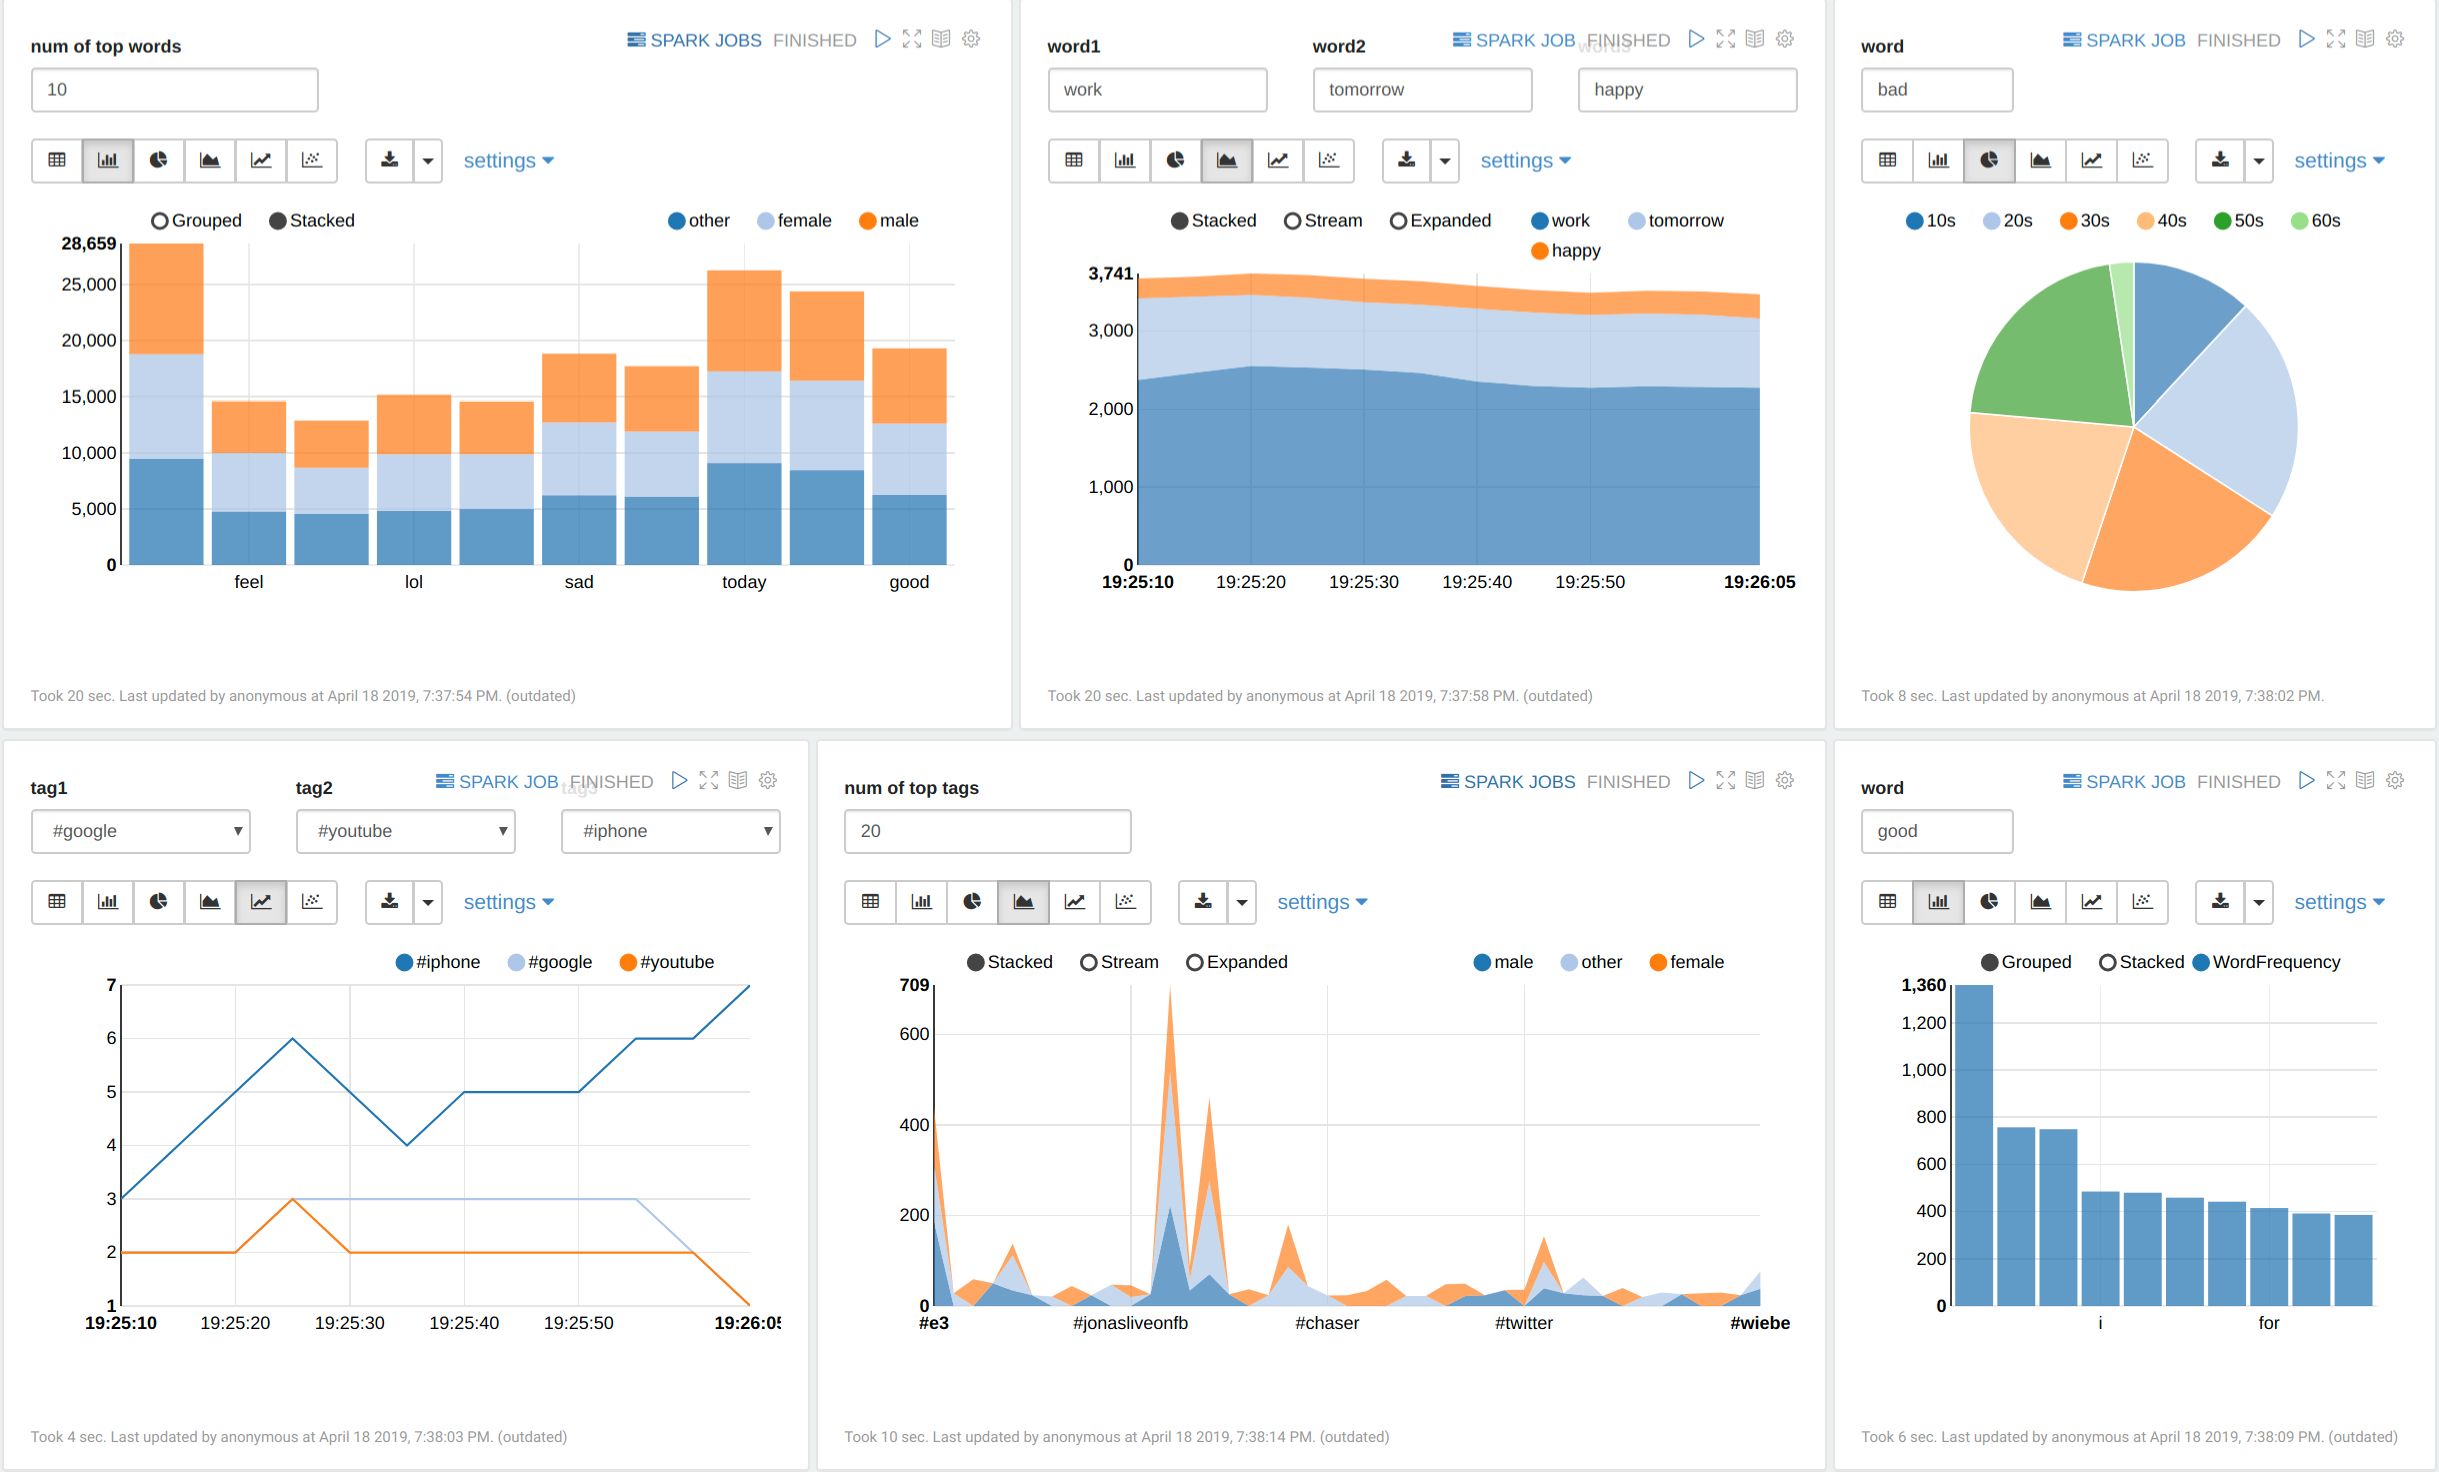
\includegraphics[width=\textwidth]{dashboard.png}
    \caption{General look of the final dashboard. Note that gender and age data is randomly made up, so don't take it seriously :)}
    \label{fig:dashboard} 
\end{figure}

The dashboard is implemented in a stand alone spark context, which loads newest intermediate data from the intermediate result files (it could be from HDFS too, but in order to make it compatible with the lightning-viz library in the previous job, we store them as local file). The spark program reads the text files and performs some simple joining/filtering work, producing a DataFrame object at the end (see the GitHub repository for detailed codes). In the next Zeppelin paragraph, the DF can then be further used by invoking some spark SQL queries, which produces those charts that make up the dashboard. 

\subsubsection{Interactivity}
As can be seen in Fig. ~\ref{fig:dashboard}, the spark paragraph and most of the plotting graph comes with interactive widgets, including reading user input, a list to choose from or selection boxes, see more details when the mouse hovers on a part, or interact with graph elements such as labels. For example, after seeing the popular words/topics one can further input the words of interest to check how fast they are growing, as well as the age/gender distribution when investigating the trend of outbreak news. On the dashboard, we designed the following interactive features:

\begin{enumerate}
    \item Aggregated word frequency in the past 1 minute. User can input the number of N which will affect the number of first-N words been displayed. Also clicking on the gender tags can display/hide this information (same below).
    \item User can choose 1-3 words they are interested in and check the trend in the past minute. Usually they may pick words from the first graph (highest frequency?)
    \item User pick a word and check the age distribution.
    \item User pick three twitter tags and check the trend in the past minutes.
    \item Aggregated tag frequency in the past minute. Similar to dash 1.
    \item User select a word and the plot shows its most related word.
\end{enumerate}

Besides the content of interest in the charts, the charts themselves, are actually flexible. A GIF in our GitHub repository shows how the format and data groups of can be changed. Also, all the charts can have their types changed among pie chart, histogram, line, scatter and accumulative, all at running time.

\subsubsection{Update with streaming data}
This dashboard, however, is less real-time than the previous figure, therefore does not meet our requirement of streaming plotting. The way we use to work around this issue is adding a button on the web page, which just utilizes some augluarJS automation tricks to rerun the spark job and plotting. Since the spark job retrieves data from the most recent N time windows (updated every 10 seconds) where N can be changed by user, whenever the button is clicked, the most recent data is processed and plotted, so in this way we "simulate" the streaming plotting.

\section{Conclusion}
In this project we built a tweet data collection-streaming-processing-visualization system with decent robustness and flexibility. If replaced with some other business or social media data (text), it would become an ad-hoc analysis platform which allows users to easily track the trend of outbreak news or quickly focus on the bursty issues. The user-friendly and highly-customize visualization interface can also apply to various analysis scenarios. 

Some problems must be overcome if we would like to deploy this into a more real-life environment, including tuning the distributed instead of local Flume-Kafka architecture, and visualizing the data fluently directly from HDFS as the nature of real production environment. Also, although as mentioned above, twitter API does not provide us with enough streaming data, we will try to use some web crawlers to fetch some newer data into our data set, so we can perform more realistic analysis and get a better insight into the data.

\section{Copyright}
Apache\textregistered, Apache Kafka\textregistered, Apache Flume\texttrademark, Apache ZooKeeper\texttrademark, Apache Zeppelin\texttrademark names and logos are copyrights of Apache Software Foundation (ASF)\footnote{ASF Trademark Policies: http://www.apache.org/foundation/marks/}. This project includes software developed based on products from The Apache Software Foundation (http://www.apache.org/).

\begin{acks}
We sincerely thank Prof. Adam Roegiest's generous advice on our proposal and guidance in this project.
\end{acks}

%
% The next two lines define the bibliography style to be used, and the bibliography file.
\bibliographystyle{ACM-Reference-Format}
\bibliography{ref}

\end{document}
